\documentclass[border=0.2cm]{standalone}
\usepackage{tikz}
\usetikzlibrary{shapes.geometric}
\usetikzlibrary{shapes}

\begin{document}
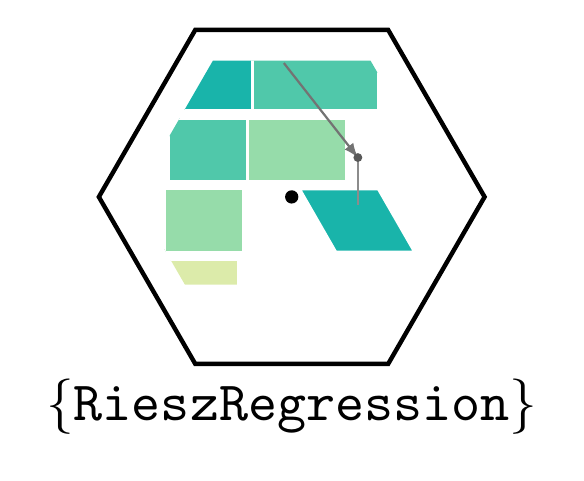
\begin{tikzpicture}[scale=2]

  % Hex clip (same structure as your nadir logo)
  \begin{scope}
    \clip ( {cos(60*1)} , {sin(60*1)} )
      -- ( {cos(60*2)} , {sin(60*2)} )
      -- ( {cos(60*3)} , {sin(60*3)} )
      -- ( {cos(60*4)} , {sin(60*4)} )
      -- ( {cos(60*5)} , {sin(60*5)} )
      -- ( {cos(60*6)} , {sin(60*6)} )
      -- cycle;

    % Optional subtle background wash (comment out if you want pure white)
    % \fill[black!2] (-2,-2) rectangle (2,2);

    % --- "Recursive blocks" forming a stylized R ---
    % Geometry settings
    % The blocks are rectangles with small offsets; together they suggest recursion/lego structure.
    % All drawn inside the clip, so you can be bold without worrying about overflow.

    % Block colors (grayscale-friendly)
    \definecolor{blockA}{RGB}{25,180,170}  % teal-ish
    \definecolor{blockB}{RGB}{80,200,170}
    \definecolor{blockC}{RGB}{150,220,170}
    \definecolor{blockD}{RGB}{220,235,170}

    % Left "spine" blocks
    \fill[blockA] (-0.75,  0.55) rectangle (-0.25,  0.95);
    \fill[blockB] (-0.78,  0.10) rectangle (-0.28,  0.50);
    \fill[blockC] (-0.81, -0.35) rectangle (-0.31,  0.05);
    \fill[blockD] (-0.84, -0.80) rectangle (-0.34, -0.40);

    % Rounded edges illusion (thin white lines)
    \draw[white, line width=1.0pt] (-0.75,  0.55) rectangle (-0.25,  0.95);
    \draw[white, line width=1.0pt] (-0.78,  0.10) rectangle (-0.28,  0.50);
    \draw[white, line width=1.0pt] (-0.81, -0.35) rectangle (-0.31,  0.05);
    \draw[white, line width=1.0pt] (-0.84, -0.80) rectangle (-0.34, -0.40);

    % Upper "bowl" of the R (two blocks extending right)
    \fill[blockB] (-0.25, 0.55) rectangle (0.55, 0.95);
    \fill[blockC] (-0.28, 0.10) rectangle (0.35, 0.50);

    \draw[white, line width=1.0pt] (-0.25, 0.55) rectangle (0.55, 0.95);
    \draw[white, line width=1.0pt] (-0.28, 0.10) rectangle (0.35, 0.50);

    % Diagonal "leg" of the R (a slanted parallelogram-like block)
    \fill[blockA]
      (0.05, 0.05) -- (0.55, 0.05) -- (0.78, -0.35) -- (0.28, -0.35) -- cycle;
    \draw[white, line width=1.0pt]
      (0.05, 0.05) -- (0.55, 0.05) -- (0.78, -0.35) -- (0.28, -0.35) -- cycle;

    % --- Subtle "projection" motif (Riesz / inner product) ---
    % A thin arrow and a perpendicular drop-line to hint at projection/operator geometry.
    \draw[black!55, line width=0.8pt, -latex] (-0.05, 0.85) -- (0.42, 0.25);
    \draw[black!45, line width=0.7pt] (0.42, 0.25) -- (0.42, -0.05);
    \fill[black!65] (0.42, 0.25) circle (0.8pt);

    % A small central "psi" dot (kept minimal)
    \fill[black] (0,0) circle (1.2pt);

  \end{scope}

  % Hex outline (same as your template)
  \draw[black, thick] (0,0) node[regular polygon, regular polygon sides=6, inner sep=1.5cm] {};
  \node[ultra thick, regular polygon, draw, regular polygon sides=6, inner sep=1.5cm] at (0,0) {};

  % Bottom label plate (same silhouette as your template)
  \fill[draw=white,color=white] (-.85,-.56) -- (.85,-.56) -- (.52, -.98) -- (-.52, -.98) -- cycle;
  \node [scale=2.0, color=black] at (0,-1.33) {\texttt{\{RieszRegression\}}};

\end{tikzpicture}
\end{document}

